\begin{tframe}{Literature of Knowledge Graphs}
    A KG refers to a semantic network graph which is consisted of diverse entities, concepts, and relationships in the real world. %(\cite{Hogan2021});
    %It is used to formally describe various things and their associations in the real world.
    \vspace{0.2cm}

    \textbf{Applications}: Social networks, IoT, Healthcare, Search Engines\ldots
    \vspace{0.2cm}

    \begin{minipage}[t]{.5\linewidth}
        \textbf{Benefits of KGs:}
        \begin{adv}
            \item Data unification;
            \item Easy availability;
            \item Semantic meaning;
            \item Easier integration;
            %\item Visualization~of~knowledge~flow;
            \item Discovery of hidden patterns;
            \item Faster decision making.
        \end{adv}
    \end{minipage}%
    \hfill%
    \begin{minipage}[t]{.5\linewidth}
        \textbf{Challenges of KGs:}
        \begin{disadv}
            \item Knowledge graph embeddings;
            \item Knowledge acquisition;
            \item Knowledge completion;
            \item Knowledge fusion;
            \item Knowledge reasoning.
        \end{disadv}
    \end{minipage}
\end{tframe}
%
% \begin{tframe}{Application of KGs}
%     \begin{figure}[htbp]
%         \centering
%      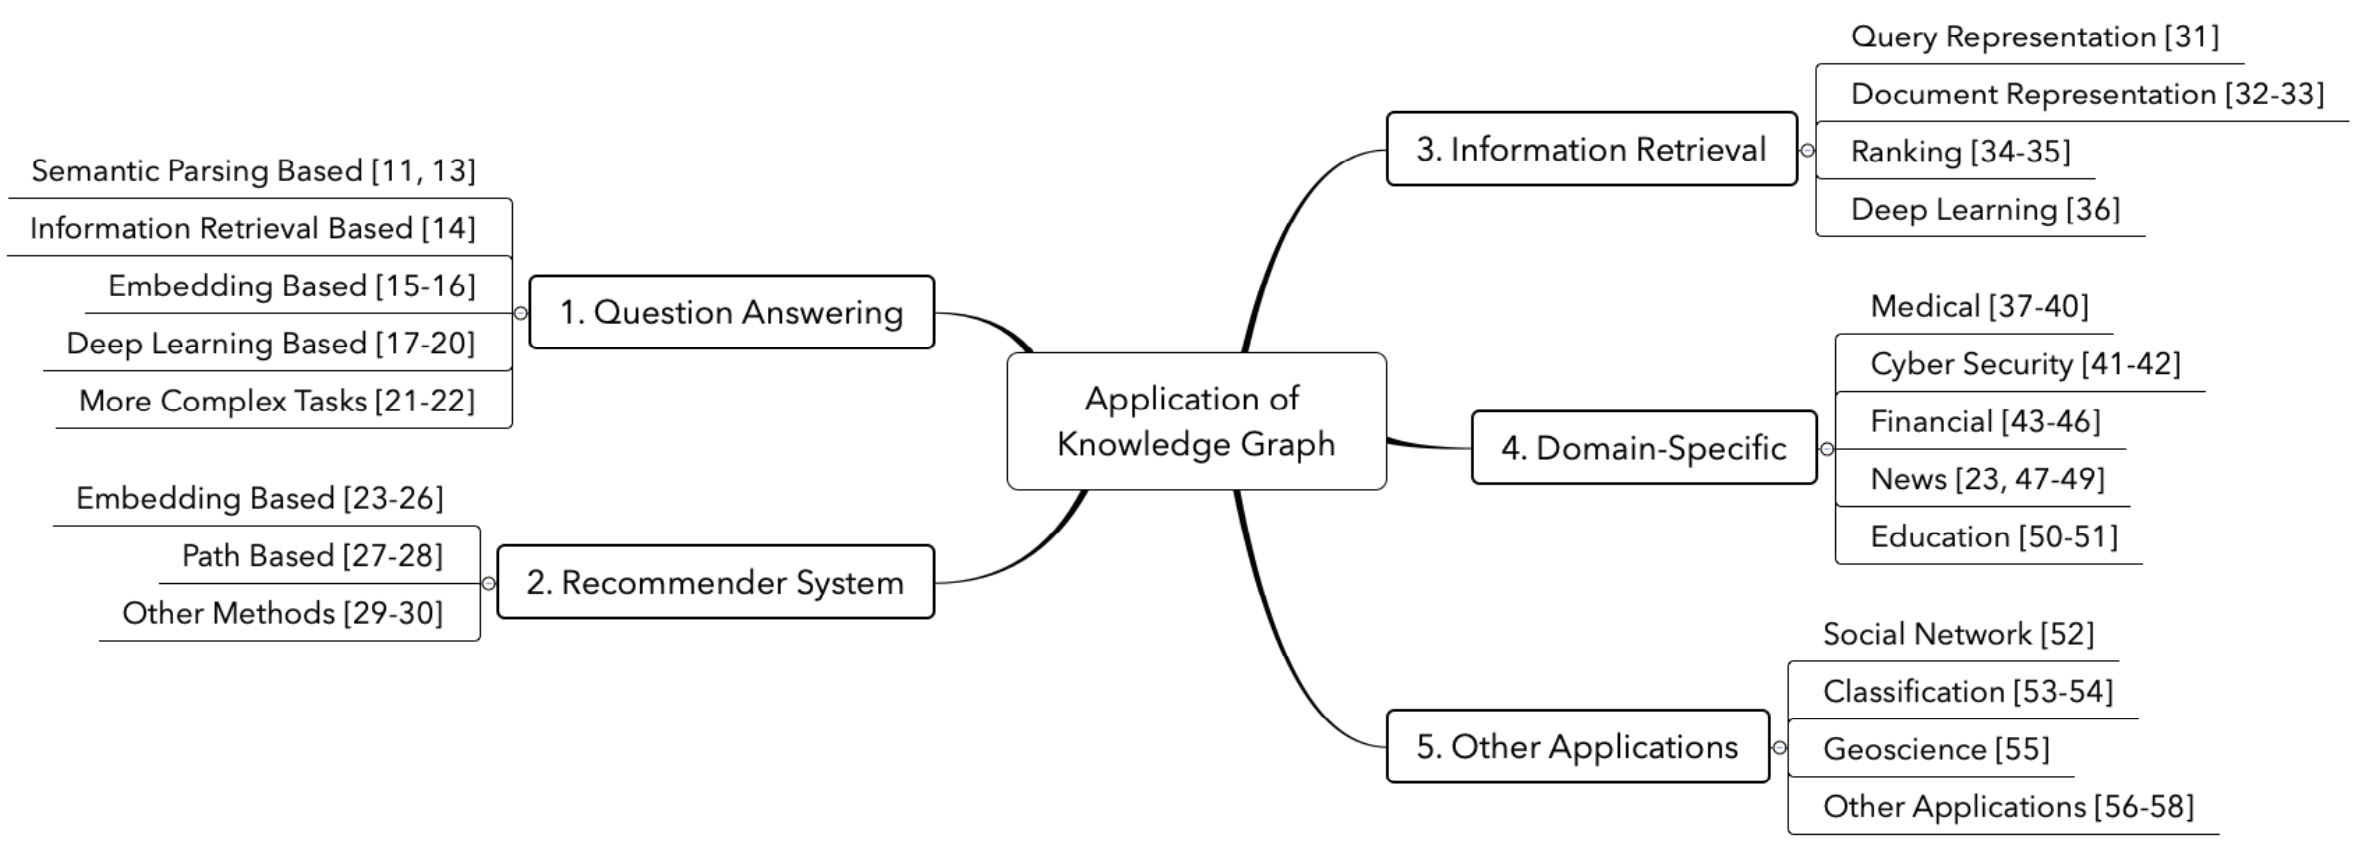
\includegraphics[width=0.9\textwidth]{../img/literature-review/application-field-kg.png}
%      \caption{Application fields of KGs (\cite{Zou2020})}
%     \end{figure}
% \end{tframe}